%%%%%%%%%%%%%%%%%%%%%%%%%%%%%%%%%%%%%%%%%%%%%%
%                insertmeeting
% 1) Title (something creative & funny?)
% 2) Date (MM/DD/YYYY)
% 3) Location (ex. Hagerty High School)
% 4) People/Committees Present 
% 5) Picture 
% 6) Start Time & Stop Time (ex. 12:30AM to 4:30PM)
%%%%%%%%%%%%%%%%%%%%%%%%%%%%%%%%%%%%%%%%%%%%%%
\insertmeeting 
	{Party Like It's 1989} 
	{03/17/22} 
	{Hagerty High School}
	{James, Jensen, Nathan, Ritam}
	{Images/RobotPics/robot.jpg}
	{2:30 - 4:30}
	
\hhscommittee{Software}
\noindent\hfil\rule{\textwidth}{.4pt}\hfil
\subsubsection*{Goals}
\begin{itemize}
    \item Improve the arm movement PID 

\end{itemize} 

\noindent\hfil\rule{\textwidth}{.4pt}\hfil

\subsubsection*{Accomplishments}
Today our mentor suggested changing the way we use the PID on the arm. Although our SimpleMovingAverage from last time greatly improved our consistency, we might be able to make it better. Currently, we used a positional PID and adjusting for gravity by subtracing a constant. One suggestion we had was to use a velocity PID when moving the arm far away from the target, then switching to a positional PID when the arm approaches its target position. In theory, this solution should help make the arm's movement smoother throughout the entire range of motion. However, we encountered a few problems with this approach. For example, the arm seemed to oscillate heavily when we switched to using the positional PID at values close to the target when compared to using a pure positional PID throughout. Even when we moved the coefficients to extremely low values, the arm movement never seemed as smooth. One possibility that the velocity PID was telling the arm to move too quickly, making it slightly more difficult for the positional PID to account for the higher momentum. 


\begin{figure}[htp]
\centering
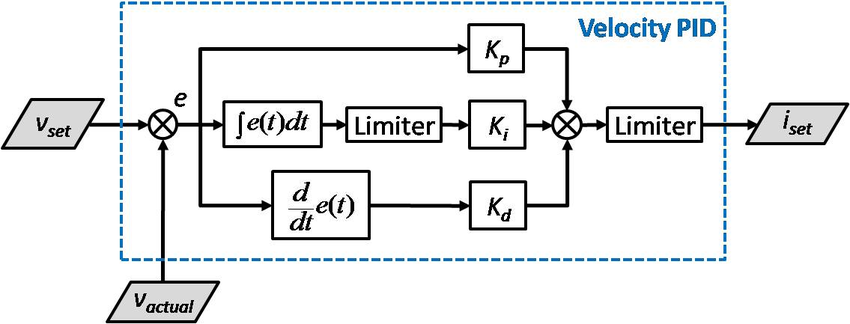
\includegraphics[width=0.95\textwidth, angle=0]{Meetings/March/03-17-22/03-17-22 1.png}
\caption{A flowchart showing the basic idea of a velocity PID that we would use.}
\label{fig:031722_1}
\end{figure}



\whatsnext{
\begin{itemize}
    \item Explore more ways to improve the arm movement. 
\end{itemize} 
}

